% Trước khi giải thích về thuật toán tối ưu hóa đa nhiệm 2 - MFEAII, tôi xin giải thích về nền tảng của nó, thuật toán tối ưu hóa đa nhiệm 1 - MFEAI
\label{mfeai}

Tiến hóa đa nhiệm như giải thích về MFO ở trên, MFEA-I áp dụng ý tưởng này để giải quyết một tập $K$ tác vụ đồng thời. Mỗi tác vụ $k \in \{1, ..., K\}$ sẽ có không gian tìm kiếm riêng là $X_k$ và hàm mục tiêu riêng là $F_k(x)$. Tuy nhiên MFEA-I chỉ sử dụng một quần thể để mã hóa toàn bộ $K$ không gian tìm kiếm đó. Do vậy tất cả các vật liệu di truyền từ các tác vụ khác nhau sẽ được mã hóa vào chung trong một không gian tìm kiếm chung. Các giải pháp từ các tác vụ khác nhau sẽ được đưa về một cấu trúc giống nhau để có thể sử dụng, kết hợp. Trong mỗi lần đánh giá, véc-tơ biểu diễn của tác vụ $k$ sẽ được giải mã từ không gian tìm kiếm chung về không gian tìm kiếm riêng của nó và tính giá trị của hàm mục tiêu. Một định nghĩa về không gian tìm kiếm chung thường được sử dụng đó là gán bằng giá trị của không gian tìm kiếm hay số chiều của tác vụ dài nhất. 

Một số định nghĩa quan trọng trong MFEA-I được đề xuất như sau:

\begin{definition}{\textbf{Giá trị thích nghi đơn nhiệm}} (thuật ngữ gốc: \emph{factorial cost}) $\Psi^i_j$ của cá thể $p_i$ đối với tác vụ cần tối ưu $T_j$ được tính bởi công thức $\Psi^i_j=\lambda\cdot\sigma^i_j +f^i_j$, với $\lambda$ là hệ số phạt lớn, $f^i_j$ và $\sigma^i_j$ lần lượt là giá trị hàm mục tiêu và tổng giá trị vi phạm ràng buộc tương ứng với mỗi $p_i$ và $T_j$. Theo đó $p_i$ là giải pháp khả thi với $T_j$ (giá trị vi phạm ràng buộc bằng 0), chúng ta có $\Psi^i_j=f^i_j$.
\label{def:factorial_cost}
\end{definition}

\begin{definition}{\textbf{Xếp hạng đơn nhiệm}} (thuật ngữ gốc: \emph{factorial rank}) $r^i_j$ của cá thể $p_i$ trên tác vụ $T_j$ đơn giản là chỉ số của $p_i$ trong danh sách các cá thể của quần thể được sắp xếp theo thứ tự giảm dần của $\Psi_j$.
\label{def:factorial_rank}
\end{definition}


Trong trường hợp $\Psi^a_j=\Psi^b_j$ với một cặp cá thể $p_a$ and $p_b$, có thể ngẫu nhiên lựa chọn để gán các giá trị \emph{xếp hạng đơn nhiệm}. Tuy nhiên vì hiệu suất của 2 cá thể là tương đương tại tác vụ $j^{th}$ nên ta sẽ gán nhãn nó như là đối tác $j$.
\begin{definition}{\textbf{Chỉ số kĩ năng}} (thuật ngữ gốc: \emph{skill factor}) $\tau_i$ của cá thể $p_i$ là một tác vụ trong số tất cả các tác vụ của MFO với điều kiện là cá thể $p_i$ có hiệu quả nhất trên tác vụ này. Công thức: $\tau_i = argmin_j{r^i_j}$ với $j \in {1, 2, ..., K}$
\label{def:skill_factor}
\end{definition}

\begin{definition}{\textbf{Độ thích nghi vô hướng}} (thuật ngữ gốc: \emph{scalar fitness}) $\phi_i$ của cá thể $p_i$ dựa vào danh sách các factorial ranks ${r^i_1, r^i_2, ..., r^i_K}$ của cá thể $p_i$ đối với tất cả các tác vụ. Công thức: $\varphi_{i}=1/\min_{j\in\{1,\ldots,K\}}\left\{r_{j}^{i}\right\}$.
\label{def:scalar_fitness}
\end{definition}

Trên cơ sở này Gupta, Ong and Feng đề xuất lược đồ giải thuật cho MFEA-I như hình \ref{mfea-flow} \cite{gupta2016multifactorial}.
\begin{figure}
    \centering
    \fbox{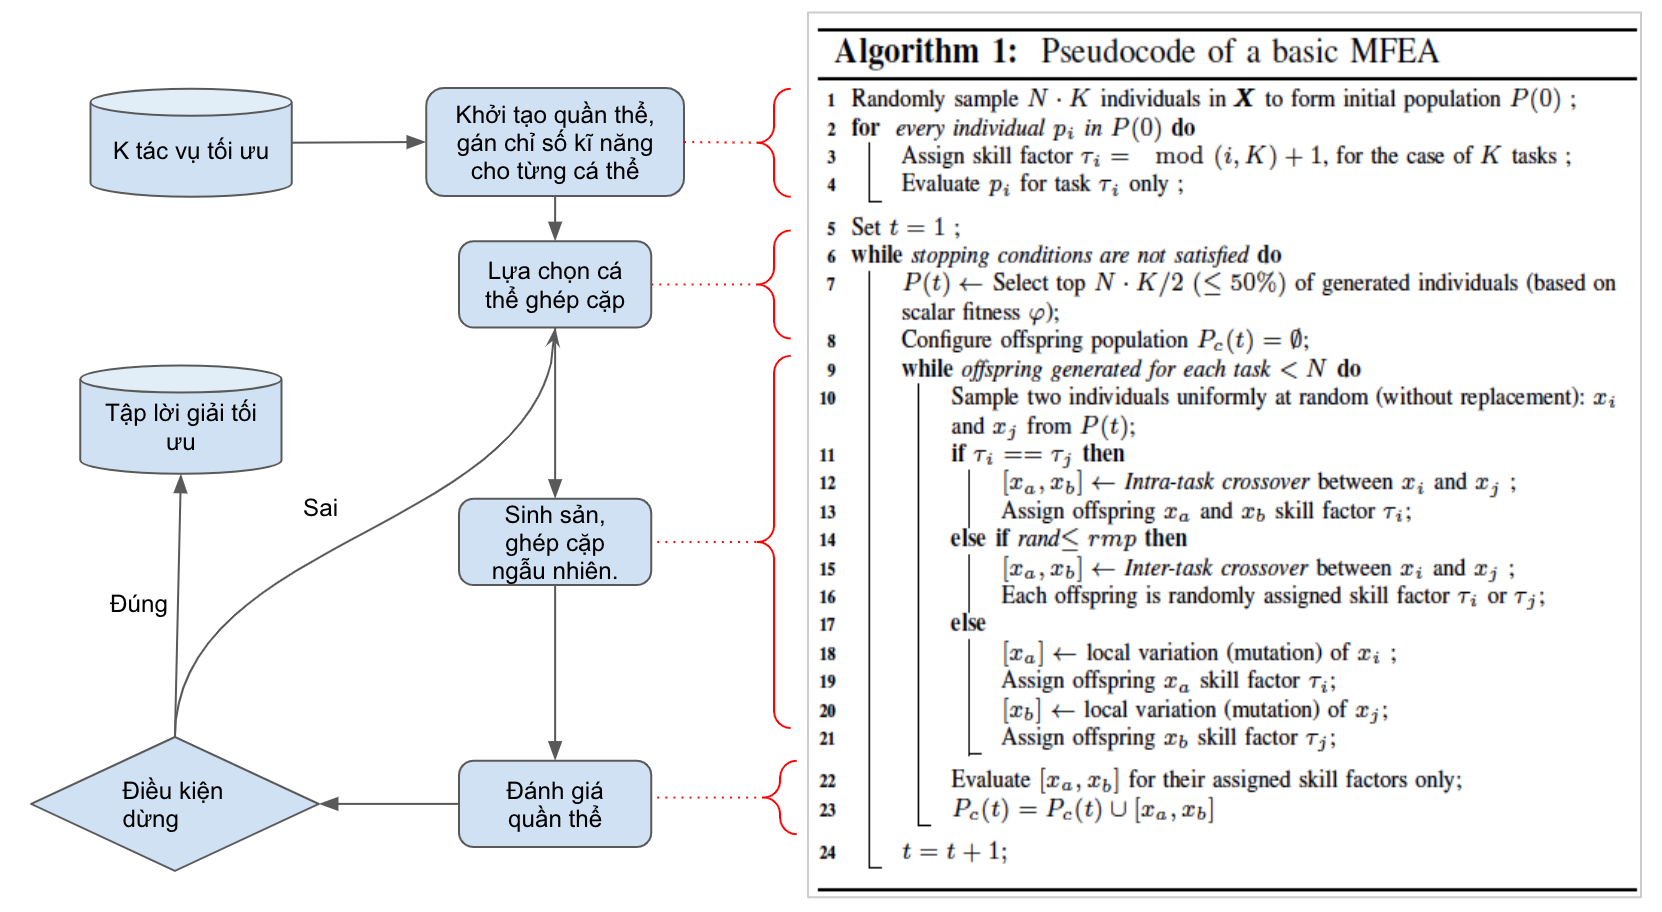
\includegraphics[width=0.85\linewidth]{thesis/images/mfea-alg.png}}
    \caption{Lược đồ giải thuật tiến hóa đa nhiệm MFEA-I \cite{gupta2016multifactorial}}
    \label{mfea-flow}
\end{figure}

Trong đó điểm khác biệt lớn nhất của MFEA-I so với thuật toán tiến hóa thông thường được mô tả tại \ref{section:cea} là cho phép lai ghép cá thể của các bài toán khác nhau theo một xác suất ghép cặp ngẫu nhiên (thuật ngữ gốc: \emph{random mating propability - rmp}). Phép lai ghép ngẫu nhiên đa nhiệm này đem đến một khả năng chia sẻ các gen tốt gữa các bài toán tối ưu hóa để đồng thời giải quyết cùng lúc chúng với tốc độ hội tụ nhanh hơn. 

Tuy nhiên, liệu việc kết hợp các lời giải của các bài toán tối ưu hóa khác nhau thì có sinh ra lời giải tốt hay không? Hoặc ít nhất cũng cần chỉ ra được trong trường hợp nào thì tốt, trường hợp nào thì không tốt. Các mục tiếp theo trong đồ án sẽ làm rõ hơn về vấn đề này.
